\section{Spectral element method on non conforming meshes}
Equation \ref{eq:weakform} is the problem we will be attempting to solve. However, the equation must still hold for every function $v \in H_0^1(\Omega)$. This section presents the method used for the discretization of the problem, namely the spectral element method on a non conforming mesh. 

The first part of the task is the discretization of the domain $\Omega$. As explained in the introduction, we will use non conforming meshes. So we will present such meshes, present their particularities and explain how we will handle them.   

The second part of the task is the discretization of equation \ref{eq:weakform}. The method here presented is the spectral element method, which consists of using high degree piece-wise polynomials as basis functions. We will at first present the one dimensional basis functions used and the location of the nodes on the 1D reference element. We will then explain how to handle the hanging nodes whose presence will arise due to the AMR. We will finally explain how to build the linear system ($Au= b$) to solve the discrete problem and how to efficiently perform a matrix-vector product with said matrix $A$.

\subsection{Discretization of the domain}

Let us first tackle the discretization of the domain. In classical AMR, the mesh depends on the problem to solve and the refinement is performed to obtain the fact that the error committed on each quadrant is roughly the same (\textcolor{red}{ref here}). But that is not the focus of the work done here. Instead, let us assume that we already have a mesh $G$ consisting of unstructured quadrilaterals (denoted $\Omega_e$) and that might be non conforming, i.e. where we have the presence of hanging nodes. As always, we have : 

\begin{align*}
G &= \bigcup\limits_{e} \Omega_e\\
\Omega_i \cap \Omega_j &= \emptyset &\text{if $i\neq j$}
\end{align*}

\begin{figure}
\centering
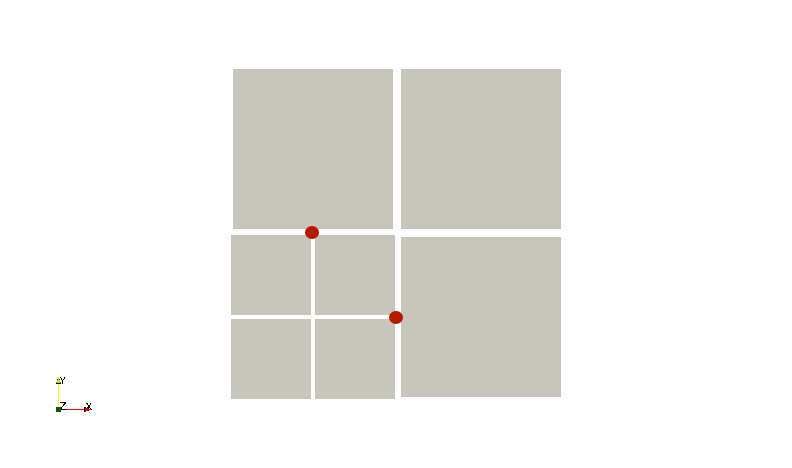
\includegraphics[scale=0.45]{Theory/hang_ex.png}
\caption{Example of a legal non conforming mesh. We can see that we have two hanging nodes in red since they are not vertices of the bigger quadrants neighboring them.}
\label{hang_ex}
\end{figure}

We can define a hanging node as being a node that is not shared between all its neighboring quadrants. Figure \ref{hang_ex} shows an example of a mesh containing hanging nodes. We can see that the vertices in red are hanging nodes since they are vertices of the smaller quadrants neighboring them but not of the bigger quadrants neighboring them. Those nodes will require a special treatment in the spectral element method. 

\begin{figure}
\centering
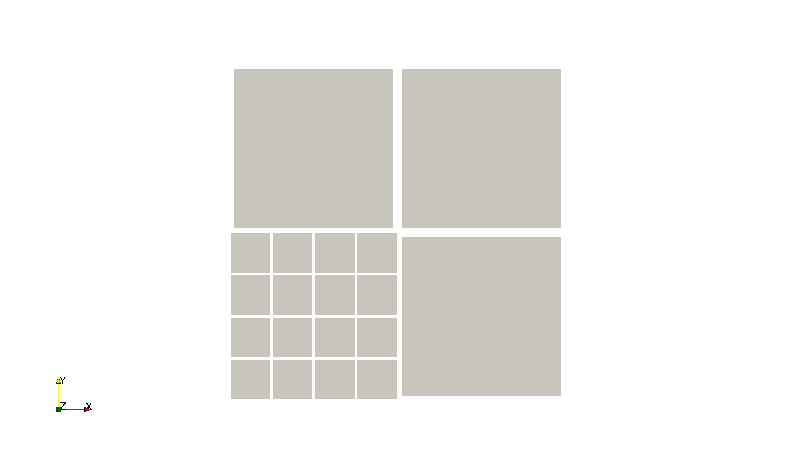
\includegraphics[scale=0.45]{Theory/hang_illegal.png}
\caption{Example of an illegal non conforming mesh. We can see that the top left quadrant has four neighbors through its south edge while we imposed a maximum of two. }
\label{hang_illegal}
\end{figure}

We have however one restriction to make on the mesh. We will allow two neighboring quadrants to have only one level of difference in the refinement. This means that the number of neighbors of a quadrant through a given edge is maximum two. Figure \ref{hang_illegal} shows an example of an illegal non conforming mesh. We can see that on that mesh the top left quadrant has four neighbors through its south edge. Handling all possibilities of hanging faces is impossible and that is why we (and the vast majority of others) consider as illegal meshes such as the one presented in figure \ref{hang_illegal}.

Once we have our mesh, it is clear that we can compute the integral of any scalar function $g$ as the sum of integrals on the quadrants. Formally, we have :  

\begin{align}
\int_\Omega g\:dxdy = \sum_e \int_{\Omega_e} g\:dxdy \label{eq:int}
\end{align}

All the integrals we compute will be performed quadrant by quadrant and then summed. 

\subsection{Discretization of equation \ref{eq:weakform}}

Since equation \ref{eq:weakform} must hold for every function $v \in H_0^1(\Omega)$, it is not very practical. We will therefore restrict ourselves to $V^h \subset H_0^1(\Omega)$, where $V^h$ has a finite dimension. Let us denote the functions that form the basis of $V^h$ by $\phi_1,..., \phi_N$ (therefore, the space $V^h$ is of dimension $N$). We will define explicitly those basis functions later. 

Using Galerkin approximation, we will also restrict our search of the solution to $V^h$. Let us denote this solution $u^h$. Therefore, we have that : 

$$u^h = \sum_{j=1}^N u_j \phi_j $$

Asking equation \ref{eq:weakform} to be satisfied for every function in $V^h$ is equivalent to ask it to be satisfied for every function of its basis. As a results, the discretized version of equation \ref{eq:weakform} is given by : 

\begin{align}
\sum_{j = 1}^N \int_\Omega \nabla \phi_i \cdot \nabla \phi_j \:dxdy \: u_j &= -\int_\Omega f\phi_i \:dxdy &\text{for $i=1,...,N$} 
\end{align}

Solving this to get the nodal values $u_j$ is actually solving a linear system of equations $\textbf{Au}=\textbf{b}$ where we define : 

\begin{align}
A_{ij} &= \int_\Omega \nabla \phi_i \cdot \nabla \phi_j \:dxdy \label{eq:A}\\
b_i &= -\int_\Omega f\phi_i \:dxdy \label{eq:b}
\end{align}

Those integral will be performed using equation \ref{eq:int}.

\subsection{Basis functions on the reference element and Gauss-Lobatto-Legendre nodes}

As shows equations \ref{eq:A} and \ref{eq:b}, we need to compute integrals to solve the problem. Here, we will perform the integration using Gauss-Lobatto-Legendre (GLL) quadrature. The particularity of 1D GLL nodes is that they include the end points of the interval on which we compute the integral. For example, on the one dimensional reference element, it means that the GLL nodes include $\xi = -1$ and $\xi=1$. This particularity enables us to use the GLL nodes both as quadrature points and as global nodes where we compute our numerical solution. We will see later that this allows us to compute the matrix-vector product very efficiently. 

For $p+1$ GLL nodes, we can integrate exactly polynomials of degree at most $2p-1$. It is less than for the Gauss-Legendre quadrature (which achieve to integrate exactly polynomials up to order $2p+1$). The way to compute the GLL nodes and their weights is for example detailled (\textcolor{red}{ref here}). Table \ref{gll_values} shows the values for different degrees. We can see that the nodes are not uniformly distributed but they tend to cluster near the end points $\xi = -1$ and $\xi=1$.

\begin{table}
\centering
\begin{tabular}{c|cc}
\hline
 Number of nodes $p+1$ & Points $\xi_i$ & Weights $w_i$\\
 \hline
 2 & $\pm 1$ & $1$ \\
 \hline
 3 & $\pm 1$ & $\frac{1}{3}$\\
    & 0			   & $\frac{4}{3}$\\
 \hline
 4 & $\pm 1$ & $\frac{1}{6}$\\
    & $\pm \sqrt{\frac{1}{5}}$  & $\frac{5}{6}$\\
\hline
5 & $\pm 1$ & $\frac{1}{10}$\\
   & $\pm \sqrt{\frac{3}{7}}$ & $\frac{49}{90}$\\
   & $0$ & $\frac{32}{45}$\\
   \hline
\end{tabular}
\caption{Values of the GLL nodes and the associated weights on the reference one dimensional element for the first few degrees.}
\label{gll_values}
\end{table}

Let us denote the $p+1$ GLL nodes on the reference 1D element by $\xi_0$, $\xi_1$, ..., $\xi_p$. Since the GLL nodes contain the end points of the interval, we can also use them as global nodes. We will use Lagrangian polynomials for the interpolation. Let us denote them $l_0(\xi)$, $l_1(\xi)$, ... , $l_p(\xi)$. Let us recall that : 

$$ l_i(\xi) = \prod_{j=0 , j\neq i}^p \frac{\xi - \xi_j}{\xi_i  - \xi_j}$$

For the following parts of this chapter, it is very important to note that :

$$ l_i(\xi_j) = \delta_{ij} $$ 

Where $\delta_{ij}$ is to be understood as the Kronecker delta. This fact will allow us later to compute the matrix-vector product in a very efficient way. 

Let us also use this opportunity to define the derivation matrix $H$ as : 

\begin{align}
H_{ij} = l_i'(\xi_j)
\end{align}

Let us now define the basis functions on the 2D reference element. In 2D, we will use $(p+1)^2$ nodes, tensor product of the 1D GLL nodes. If we denote the 1D GLL nodes by $\xi_i^1$, the 2D nodes are thus located at :

\begin{align*}
(\xi_i, \eta_j) &= (\xi^1_i,\xi^1_j) &\text{for $i,j=0,1,...,p$}
\end{align*}

On the reference quadrant $\xi, \eta \in [-1;1]$, we have in the same way that the basis function associated with node $I$ located at $(\xi_i,\eta_j)$ is given the tensor product of the 1D basis functions : 

$$\phi_I(\xi,\eta) = l_i(\xi)l_j(\eta)$$

Thus, if we want to obtain the value of a field $u$ in the reference quadrant, whose value at node $I$ is given by $u_{ij}$, we interpolate as : 

\begin{align*}
u(\xi,\eta) = \sum_{i=0}^p\sum_{j=0}^p u_{ij}l_i(\xi)l_j(\eta)
\end{align*}

\subsection{Global basis function}

Let us first mention the distinction between global and local nodes. Each quadrant has $(p+1)^2$ local GLL nodes but that does not mean that all of them are global nodes, since some might be hanging. One solution consists to treat hanging nodes as global nodes and then add equations in the linear system $Au=b$ to enforce the continuity of the numerical solution. Another solution is to immediately enforce the continuity of the numerical solution by having continuous global basis function. This is what is done here. We will consider $N$ global nodes (that are the GLL nodes for at least one quadrant) and give them a global unique index $I = 1,...,N$. Figure \ref{global_nodes} shows the global nodes for $p=2$ on a certain mesh. 

\textcolor{red}{montrer mesh ici et aussi montrer une shape function pour p=2}


We want our global basis function $\phi_I$ to be a piece-wise polynomial of order $p$ and to have a value of exactly $1$ at global node $I$ and to be equal to $0$ on any other global node. 

In order to define such a function, we first need a mapping that goes from the 2D reference element to the actual quadrant $e$, i.e. $x^e(\xi,\eta)$ and $y^e(\xi,\eta)$ that for quadrant $e$ give the actual coordinates of any point in the reference element. Let us also define the inverse mappings $\xi^e(x,y)$ and $\eta^e(x,y)$. 

The last thing we need is is a global to local operator that gives the weight of a given global node on a local node 





